\documentclass{article}
\usepackage[utf8]{inputenc}
\usepackage{geometry}
 \geometry{
 a4paper,
 total={210mm,297mm},
 left=20mm,
 right=20mm,
 top=20mm,
 bottom=20mm,
 }
 
\usepackage{float}
\usepackage{graphicx}
\usepackage{multirow}

 
\pdfinfo{
  /Title    (Building Serious Games - Design4Health)
  /Author   (Ralf Nieuwenhuizen, David Prihoda, Ismini Psychoula, Arnold Schutter, Shen Shuheng)
  /Creator  (Ralf Nieuwenhuizen, David Prihoda, Ismini Psychoula, Arnold Schutter, Shen Shuheng)
  /Producer (Ralf Nieuwenhuizen, David Prihoda, Ismini Psychoula, Arnold Schutter, Shen Shuheng)
  /Subject  (Building Serious Games)
}


%Testing report (no more than 4 pages)
%- how did you design your test session(s) aimed at assessing (i) game functionality, (ii) player
%engagement, and (iii) achievement of its proposed goals
%- description of the actual tests (test environment, demographics, etc.) and of their outcome
%- thorough discussion of the test results, in particular with regard to the three topics above, (i)-(iii)

\title{Building Serious Games: Testing Report}
\author{
	R. Nieuwenhuizen \and
    D. Prihoda  \and
	I. Psychoula \and
	A.S.C. Schutter \and
	S. Shen
 }
\date{January 2015}

\begin{document}

\maketitle

\section{Version History}
\begin{figure}[H]
  \centering
  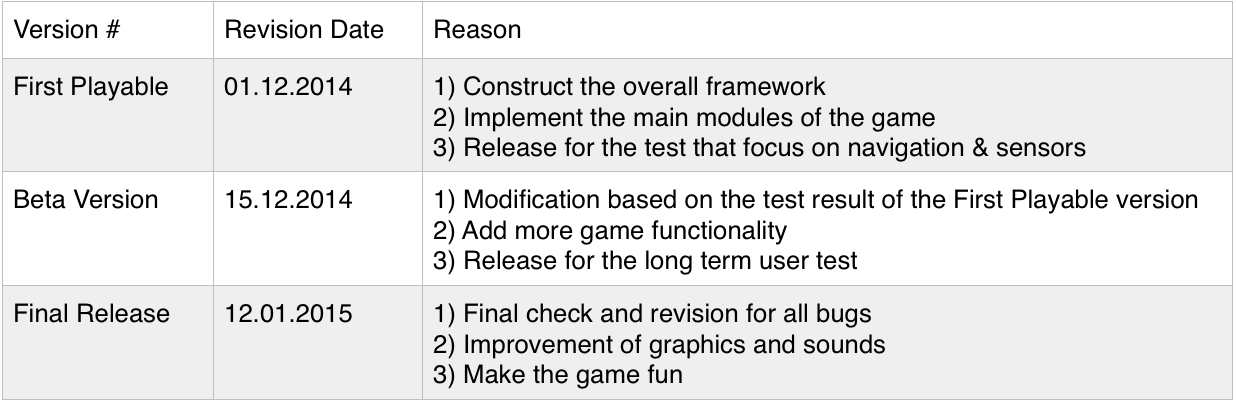
\includegraphics[width=0.85\linewidth]{VersionHistory.png}
\end{figure}

\section{Introduction}
In order to gain an objective, independent view of the end result we tested the game with several users. These users helped us to get an idea about the desires of the stakeholders. After every test session we made modifications to improve the game. We also conducted continuous self-tests during the implementation of PhysioFun to test the playability and navigation. The design and result of each test session is shown below.

\section{User Tests}
\subsection{Test for First Playable version}
For the First Playable version, the overall framework was constructed and the main modules of the game were implemented. The main focus of the test is to assess: 
\begin{itemize}
    \item{whether the navigation of the game is clear enough or not; }
    \item{whether the sensors sense the movement of the users well or not;}
    \item{whether the app responds correctly to all kinds of inputs the user triggers or not}
\end{itemize}

\subsubsection{Test Plan}
\begin{figure}[H]
  \centering
  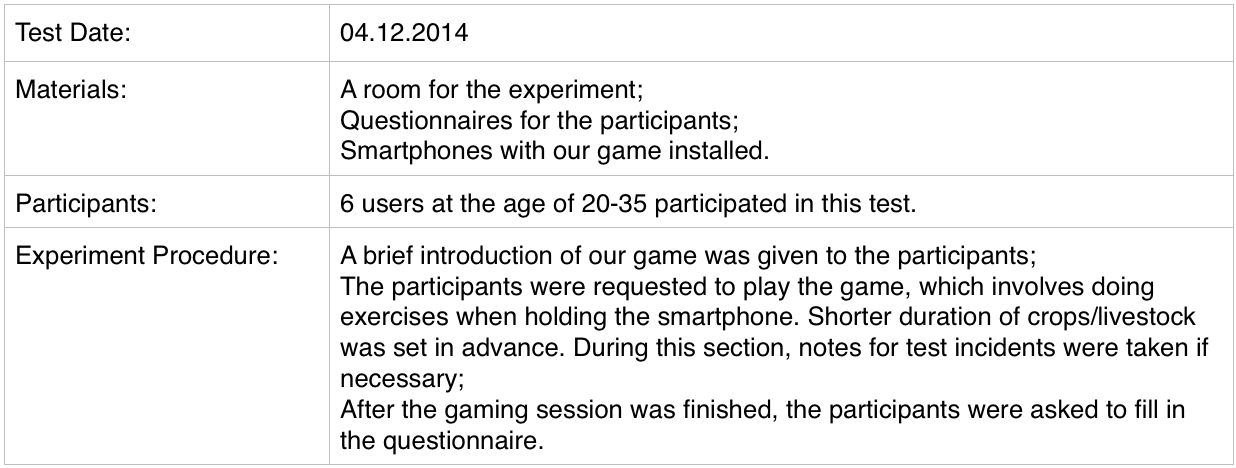
\includegraphics[width=0.9\linewidth]{TestPlan.png}
\end{figure}

\subsubsection{Summary of the Test Results}
\begin{itemize}
    \item{\textbf{Issue: Intro Screen}}
\end{itemize}

\underline{Problems/Comments:} \\\indent All the users felt confused where to begin.

\underline{Solutions:} \\\indent The navigation should be made more self-explanatory. From the beginning of the game, add a pop up screen for asking the user to select a challenge. This screen can be the instruction made by the Mentor.

\begin{itemize}
    \item{\textbf{Issue: Challenge Screen}}
\end{itemize}

\underline{Problems/Comments:} \\\indent 1. The users did not know that they have to press “select” button to pick a challenge;\\
\indent 2. The relation between the “challenge” and the “clone” is not clear.

\underline{Solutions:} \\\indent 1. Maybe it will be more intuitive in the future once we have more challenges that form into a list, from which you can choose a challenge;\\
\indent 2. Change the challenge screen into several steps. The sketch is as follows:
\begin{figure}[H]
  \centering
  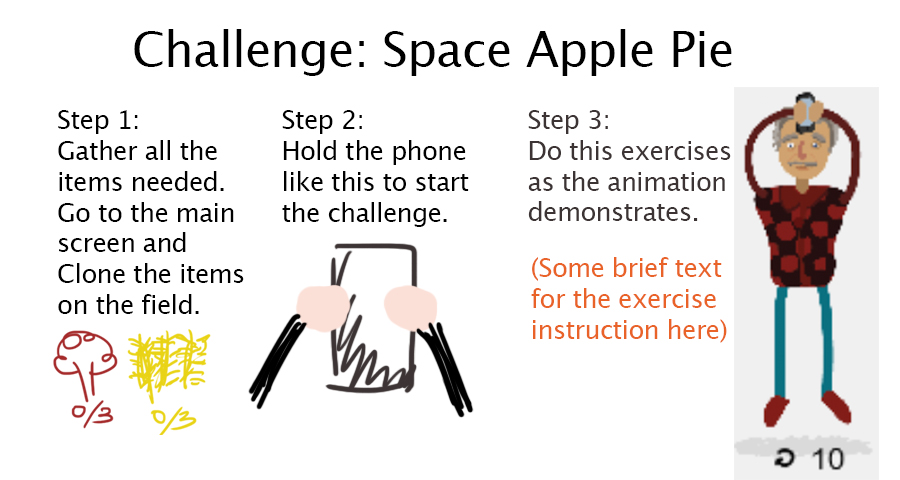
\includegraphics[width=0.6\linewidth]{challengeModify.jpg}
  \caption{Sketch for the modification of Challenge Screen}
\end{figure}

\begin{itemize}
    \item{\textbf{Issue: Exercise Screen}}
\end{itemize}

\underline{Problems/Comments:} \\\indent Once the user press the “Start” button, there’s no change for that button, i.e., no feedback is given by pressing the button.

\underline{Solutions:} \\\indent The status of the “Start” button should change, for example triggers the instruction “Do the exercise until you feel the phone buzzes”.




\subsection{Test for the Beta Version}
Modification based on the test result of the First Playable version was made. Besides, more functionalities and modules were added into the game to prepare for the long term test. The main focus of the test is to assess:
\begin{itemize}
    \item{whether the navigation of the game is clearer after the revision or not;}
    \item{whether the sensors work well for the newly added exercises or not;}
    \item{whether the graphics and sounds are suitable or not;}
    \item{whether the goal of the game is clear to the users or not and to what extent PhysioFun had motivated the users to exercise regularly}
\end{itemize}

\subsubsection{Test Plan}
\begin{figure}[H]
  \centering
  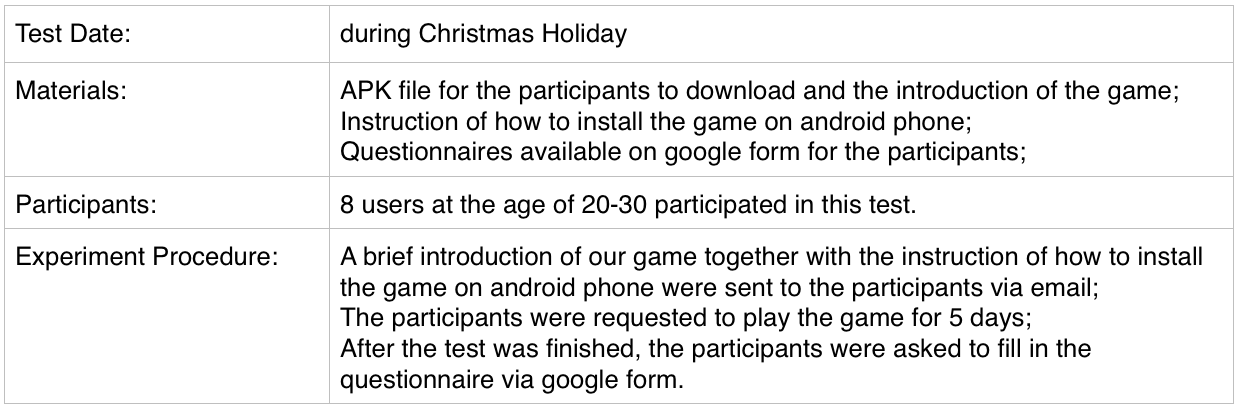
\includegraphics[width=0.9\linewidth]{TestPlan2.png}
\end{figure}


\subsubsection{Summary of the Test Results}
\textit{Some questions in the questionnaire were answered in Likert-Scale from negative attitude(0) to positive attitude(7).}
\begin{itemize}
    \item{\textbf{Issue: General}}
\end{itemize}

\underline{Problems/Comments:} \\\indent 1. About half of the subjects admitted they are not motivated to do exercises. Reasons that prevent the users from executing exercises: 1) lack of time; 2) laziness; 3) no company; \\
\indent 2. Most (7 out of 8) of the users only play games on a smart phone less than one hour everyday.

\underline{Solutions:} \\\indent 1. PhysioFun won’t occupy much time of the users, the users can always make use of their free time to get relaxed after sitting idly the whole day, especially for those people who have to work in front of the computers for a long time;\\
\indent 2. The target audience should not even include those who want to be “gym master”, we should emphasize that our target audience are those "white collars" (people who do office jobs). PhysioFun can help the white collars to prevent the occurrence of the chronic diseases like cervical spondylosis (a neck disorder).


\begin{itemize}
    \item{\textbf{Issue: Navigation}}
\end{itemize}

\underline{Problems/Comments:} \\
\indent 1. The navigation is clear to most of the users (scored 5.25 in average). Some suggestions from the users: 1) add animation to all of the exercises; 2) the instruction should disappear when clicking anywhere;\\
\indent 2. The description of the challenges is clear and understandable.

\underline{Solutions:} \\
\indent 1. Animation for all the exercises will be added in Final Version;\\
\indent 2. “To-do list” for first time use and the “Tips everyday” will be added to replace part of the instruction.


\begin{itemize}
    \item{\textbf{Issue: Exercises \& Sensors}}
\end{itemize}

\underline{Problems/Comments:} \\
\indent 1. The accuracy of the sensor scores 4.5 in average. The phone generally buzzes too soon;\\
\indent 2. Most of the users like the idea of earning money by walking/running;\\
\indent 3. The question “Do you think this game can help you to get motivated to exercise more structural?” scores 4.5 in average.

\underline{Solutions:} \\
\indent 1. Count the movement “back \& forth” as one; try some other algorithms to make the count more accurate;\\
\indent 2. The functionality of earning money by walking/running will be added;\\
\indent 3. The score for getting users motivated is moderate. The main reason for that was because of the weak quality of the graphics, which dismissed the motivation of playing.


\begin{itemize}
    \item{\textbf{Issue: Graphics \& Sounds}}
\end{itemize}

\underline{Problems/Comments:} \\\indent The graphics scores 5.125 in average. Some graphics are of weak quality; 

\underline{Solutions:} \\\indent Enhancing the graphics will be one of the main focuses in the next phase.


\begin{itemize}
    \item{\textbf{Issue: Goal}}
\end{itemize}

\underline{Problems/Comments:} \\
\indent 1. The goal of the game is clear to most of the users (scored 5.375 in average). How the level system works was not clear;\\
\indent 2. The frequency of doing exercises does not change obviously after started playing PhysioFun;\\
\indent 3. The motivation of doing exercise regularly before and after PhysioFun: scored 3.25 \& 4 in average respectively.

\underline{Solutions:} \\
\indent 1. Notify users somewhere: Level up by fulfilling all the body points shown in BODY screen;\\
\indent 2. Upon the problems 2\&3, consider to focus our user target on users who are not that serious. It’s just a game! Regarding it as a way of prevention is more reasonable.


\begin{itemize}
    \item{\textbf{Issue: Additional comments from users}}
\end{itemize}

\underline{Problems/Comments:} \\
\indent 1. More forms of rewards besides the money;\\
\indent 2. Highlight the importance of the reward (coins/money);\\
\indent 3. Simplify the instruction;

\underline{Solutions:} \\
\indent 1. Add some rewards like decorations for the farm; materials/ tools for expanding the warehouse; bombs for cleaning the barriers; fertilisers for speeding up crops or livestock, this is put on the wishlist;\\
\indent 2. Let the users realize that it’s important to gain reward (earn money) by doing exercise, otherwise it’s not possible to salvage the farm. For now the game only shows the inventory of crops/ products increase, we should also show the increase of the coins in some way, for example make an animation of rolling coins;\\
\indent 3. Now the introduction of the game is a bit rash.
After the user click “Let’s go!”, the BODY screen should show up. Then the screen should turn back to mentor again after the user close the BODY screen and shows a dialogue cloud beside the mentor, which shows the To-do list/ Tips everyday;\\


\subsection{Test for the Final Version}
For the Final Version a final check and revision for all bugs was made and the graphics and sounds were all improved. Every effort that can contribute to make the game more fun was made.

\subsubsection{Test Plan}
Test Date: 16.01.2015\\
This is the test before the release of the Final Version. We followed the principle TDD (Test-driven development) of Agile Manifesto, which helped us to refactor the code quickly. Many passers-by were requested to help with the test.

\subsubsection{Summary of the Test Results}
\textit{Only main issues are shown as follows.}

\underline{Problems/Comments:} \\
\indent 1. BODY feedback screen (WELL DONE) was not clear where to click. When there was other item behind where the user clicked, it triggered unexpected feedback;\\
\indent 2. Sensor for the exercise Sit-ups was set too sensitive;\\
\indent 3. Sound for the exercise was gone for some reason;

\underline{Solutions:} \\
\indent 1. Clicking outside the BODY feedback screen should have no effect but just shut down the screen.\\
\indent 2. The algorithm for counting the Sit-ups will be modified to a proper sampling frequency.\\
\indent 3. Revision will be made for the exercise sound bug.

\subsubsection{Test Assessment}
During the gaming session, most of the users showed their strong interest of the game and were satisfied with the graphics and the interface design. For the evaluation of whether PhysioFun can help users be more motivated to exercise structurally, it is hard to assess in short term test, but the feedback from the users were positive and encouraging. A long term test like the one for Beta Version should be conducted in the future, which will focus on the user engagement.

\end{document}
